\documentclass[a4paper]{article}
\usepackage[english]{babel}
\usepackage[utf8]{inputenc}
\usepackage[T1]{fontenc}
\usepackage{times}
\usepackage{float}
\usepackage{listings}
\usepackage[pdftex]{graphicx}
\usepackage{epstopdf}
\usepackage{pdfpages}
\usepackage{color}
\usepackage[pdftex,colorlinks=true,citecolor=black,
            pagecolor=black,linkcolor=black,menucolor=black,
            urlcolor=black]{hyperref}
\usepackage{eufrak}
\usepackage{amsmath}
\usepackage{amsbsy}
\usepackage{eucal}
%\usepackage{subfigure}
\usepackage{longtable}
\usepackage{url}
\urlstyle{same}

\usepackage{natbib}

\parindent 0mm
\parskip 3mm

\newcommand*\mean[1]{\bar{#1}}

\pdfinfo{            
          /Title      (T-61.5140 Machine Learning: Advanced Probabilistic Methods Project)
          /Author     (Ville Sillanpää, Lauri Viitanen)
          /Keywords   ()
}

\title{Classify the glass samples using Gaussian Mixture Models (GMM)}
\author{Ville Sillanpää, k84338 - Lauri Viitanen, 338853 \\ 
       {\it ville.sillanpaa@aalto.fi} -
       {\it lauri.viitanen@aalto.fi}}

\begin{document}
\maketitle
\clearpage

%\begin{figure}[]
%	\includegraphics[]{all_338853_2001.pdf}
%\end{figure}

\section{Introduction}

In this project we analyze a glass data set using both unsupervised and
supervised machine learning approaches. The glass dataset [1] has been
provided by the US Forensic Science Service and is available for download from
the UCI machine learning repository. The dataset consists of samples for 6
types of glass (class label 4 is missing in the current data set); defined in
terms of their oxide content (i.e. Na, Fe, K, etc). In particular, the dataset
contains 214 samples characterized by 9 features and the samples have been
categorized into 6 different classes of glass.

\par
The goal of the project is to classify the glass samples using Gaussian
Mixture Models (GMM) in unsupervised and supervised approaches. In the
unsupervised approach we use GMMs to find clusters from the full data set and
compare the clustering results with the ground-truth class labels that are
provided with the data set. In the supervised approach we fit a separate GMM
for each class label and evaluate the classification performance using the
fitted models on the test set. The dataset has been randomly divided into
training (75 \%) and test sets (25 \%) keeping an equal proportion of different
class instances in the training and test sets. In addition, we compare the
performance of the GMM model with the k-nearest neighbors classifier.

\section{Methodology}

\subsection{Unsupervised Approach}

DP-GMM used with Gamma prior on concentration parameter, Gaussian mean on gaussian mean and inverse wishart on covariance matrix. Model inferred using Gibbs sampling with algorithm by (insert name here). For more detailed description of model see (article).

\par
Several runs of 5000 samples were were ran. Below is a scatter plot of 5000th sample from one of the runs. The visualization was produced with multidimensional scaling. PCA was tried first, but since the first two components explained only two thirds of variation, we chose to to MDS instead. 

\begin{figure}[H]
	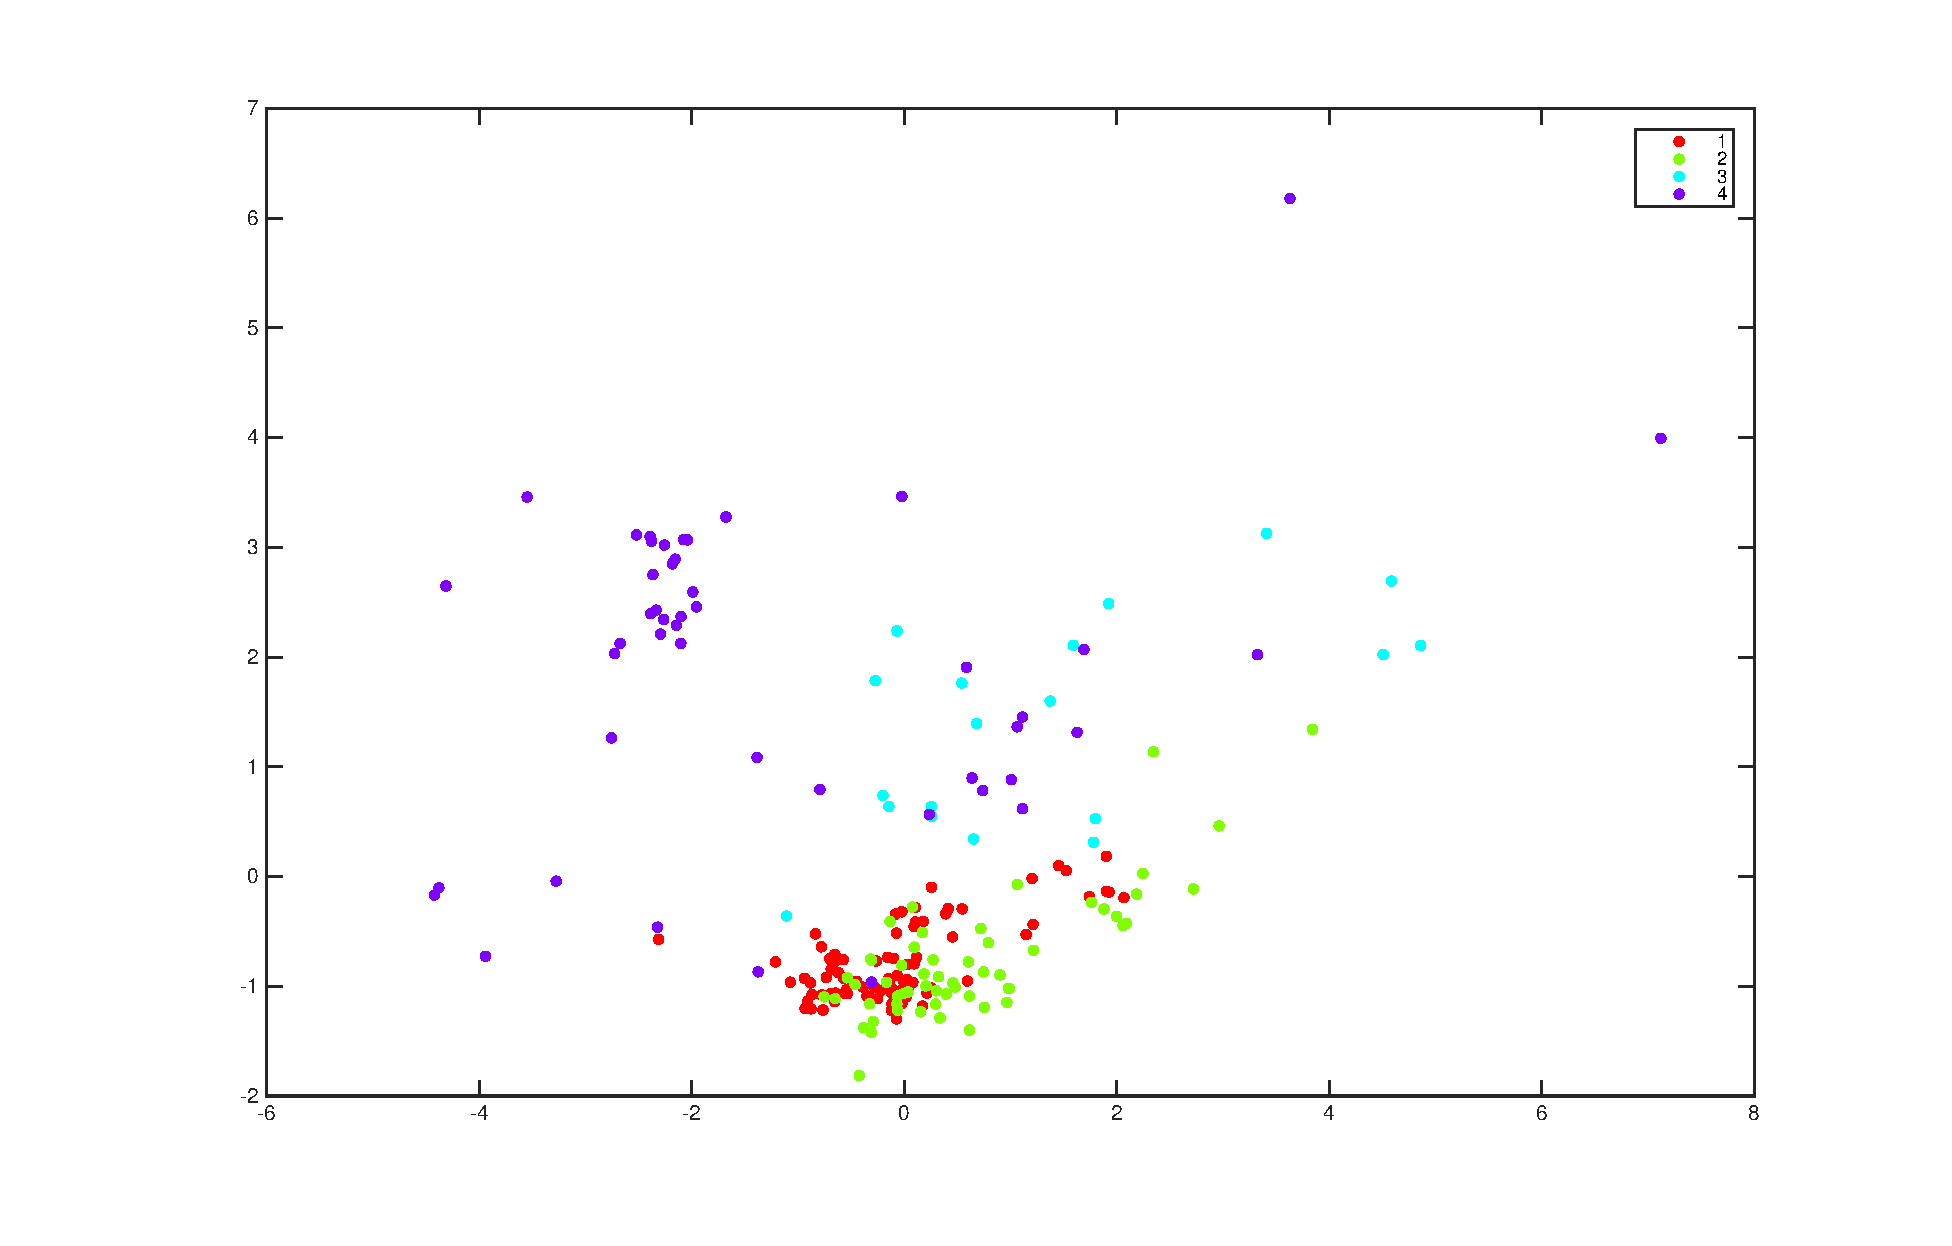
\includegraphics[scale=0.67]{5000_normalized_data_1.eps}
	\caption{MDS of unsupervised clustering}
	\label{mds_unsupervised}
\end{figure}

As you can see from \ref{fmds_unsupervised}, two dense clouds of points have been identified to belong to three clusters. This result was common to all runs. The points that are spread more sparsely were assigned to various clusters in various runs. 

\par
The runs created 3-5 clusters, with cluster assignments switching mostly within these sparsely spread points. This means that the model is able to consistently identify the two dense clouds as three different clusters, but that the model is more uncertain about the membership of the more sparse points. Based on this model it is difficult to say what clusters the sparse points belong to or that how many true labels these sparse points represent.

\par
Below is a histogram, which compares our model's label distribution to the true distribution of labels


\begin{figure}[H]
	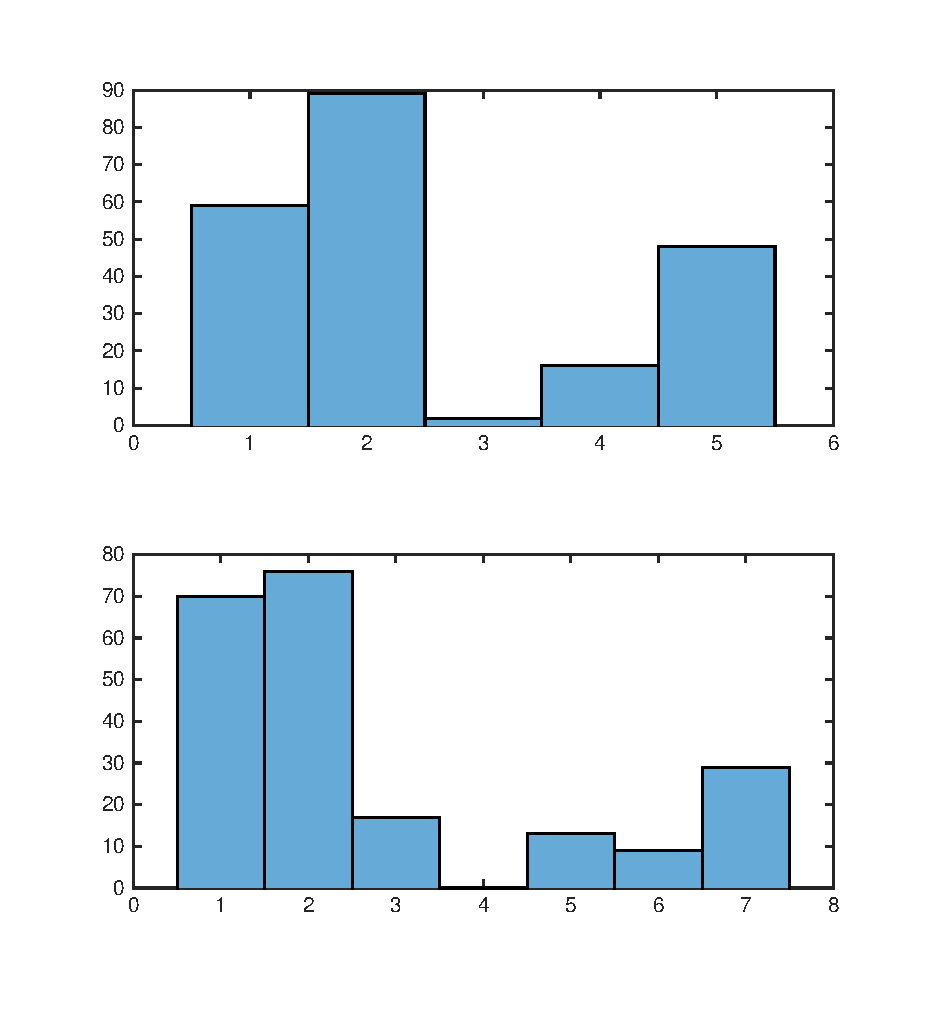
\includegraphics[scale=0.67]{histogram_comparison.eps}
	\caption{Histogram comparison of predicted versus true labels}
	\label{histogram_comparison}
\end{figure}

\par
As we can see from \ref{histogram_comparison},  There are 7 true labels as opposed to the 5 our model found. Some facts: Two large ones are identified relatively well, but remaining clusters are more troublesome. 5 and 7 might be similar.  But based on histogram its difficult to say if it is so. Let's look at MDS-visualization of true labels to confirm.

\begin{figure}[H]
	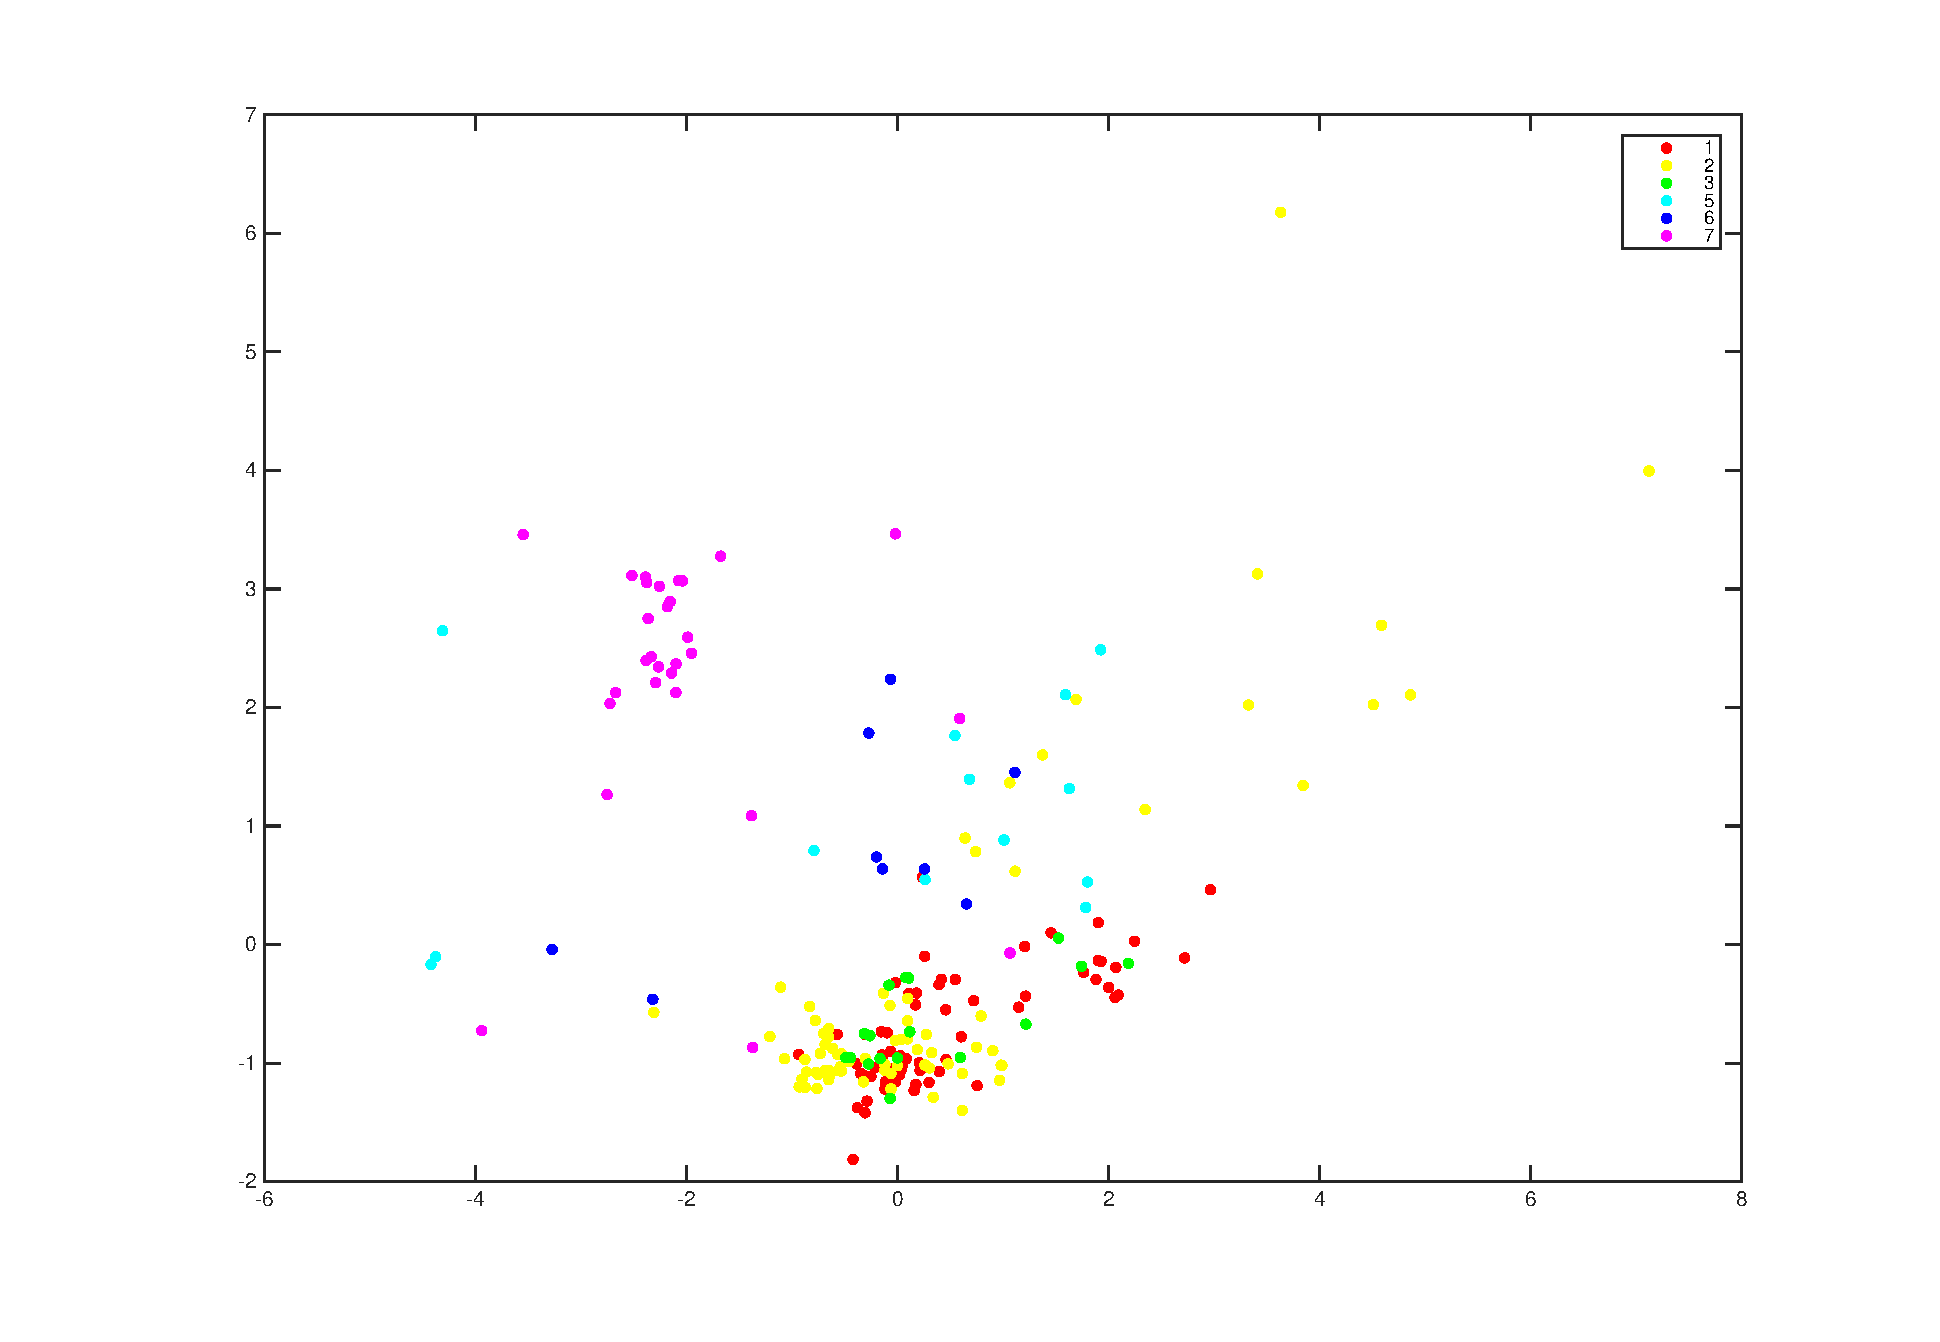
\includegraphics[scale=0.67]{MDS_true_labels.eps}
	\caption{Visualization of data using true labels}
	\label{true_labels}
\end{figure}

As we can see from \ref{true_labels}, the lower dense region is more overlapping than what our model predicts. Moreover,  quite a few of the more sparse points seem to belong into the label who is very densely concentrated (yellow). Apparently the sparse region contains observations from two additional labels. They seem to overlap so much that it is difficult to see how a gaussian mixture model would be able to find these two labels correcrly. Model and ground truth seem to agree the most about the upper dense cloud. 



\subsection{Supervised Approach}

In the supervised approach, the Gaussian mixture model is fitted to every
class label separately. The model complexities range from 2 to 10 components.
Class label 4 has no samples in the training data, class label 6 has only six
samples and class label 5 has nine samples, meaning that using more than nine
classes already drops the number of class labels from seven to four. Only
classes 1 and 2 have more than 21 samples.

\par
The GMM is fitted to the training data using the Expectation-Maximization (EM)
algorithm. The training halts after 200 iterations or if the log likelihood
has not changed enough (0.001 units) during the past few iterations (five).
The resulting fitted Gaussians are then applied to the test data of the same
classes, producing the log likelihood of the test data being produced by the
fitted GMM.

\par
VISUALIZATION HERE

\par
THEN TALK ABOUT THE MODEL COMPONENT COUNT DISTRIBUTION

\par
VISUALIZATION HERE

\section{Results}

\section{Discussion}

\par
[1] http://archive.ics.uci.edu/ml/datasets/Glass+Identification

%\begin{equation}
%\begin{aligned}
%	r[n] &= h[n] * s[n] \leftrightarrow
%		R(e^{j\omega}) = H(e^{j\omega})S(e^{j\omega}) \\
%	r[n] &= \sum_{k=-\infty}^{\infty} h[k]s[n-k] \\
%\end{aligned}
%\end{equation}

%Figure \ref{fig:100_104} shows combinations of these numbers

%\begin{figure}[H]
%	\includegraphics[scale=0.67]{m100_115_b.eps}
%	\caption{The amplitude response both in linear and logarithmic
%		(decibel) scale.}
%	\label{fig:100_115_b}
%\end{figure}

\clearpage
\appendix

\clearpage
\section*{Appendix A}\label{code:asdf}

Matlab code for asdf.

%\lstinputlisting{asdf.m}

\end{document}
